\documentclass{../crypto}
\sheet{3}
\date{30. Oktober 2015}
\usepackage{tabularx, tikz, placeins}
\usetikzlibrary{positioning}
\begin{document}

\maketitle

\section{Polynomiell Sichere Kaskadenverschlüsselung}

\subsection{}
Um ein Textpaar $(m ,c)$ zu entschlüsseln, können alle Ergebnisse der Verschlüsselungen $E_{k_i}(m)$ 
und die der Entschlüssselungen $D_{k_j}(c)$ miteinander verglichen werden. Im Fall $E_{k_i}(m)=D_{k_j}(c)$
gilt, dass ein valider Schlüssel zum Textpaar $(m, c)$ genau $(k_i, k_j)$ ist.
Es sind also nun nur genau $2|\mathcal{K}|$ Ver- bzw. Entschlüsselungsoperationen nötig.

\subsection{}
Genau wie bei a) können hier Zwischenergebnisse verglichen werden. Dabei müssen wir in einer
Richtung $|\mathcal{K}|^2$ Verschlüsselungen anwenden (eben genau $E_{k_i}(E_{k_j}(m))$), in der anderen genau 
$|K|$ viele Entschlüsselungen, $D_{k_l}(c)$.

Es sind also $|K|^2+|K|$ Ver- und Entschlüsselungsoperationen nötig.

\subsection{}
% I am not sure, if I understood this correctly...
Wählt man $k_2=k_1$, so ergibt sich direkt:

\begin{align*}
    3DES_{k_1,k_2}(m) = DES_{k_1}\left(DES_{k_2}^{-1}\left(DES_{k_1}(m)\right)\right) \\
    3DES_{k_1,k_1}(m) = DES_{k_1}\left(DES_{k_1}^{-1}\left(DES_{k_1}(m)\right)\right) \\
    3DES_{k_1,k_1}(m) = DES_{k_1}\left(m\right)
\end{align*}

Das heißt, um DES zu simulieren, muss in 3DES nur zweimal der selbe Schlüssel gewählt werden.

\section{Betriebsmodi}

\begin{tabular}{ccccccccccccc|cc}
$m_1$ & $m_2$ & $m_3$ & $m_4$ & $m_5$ & $m_6$ & $m_7$ & $m_8$ & $m_9$ & $m_{10}$ & $m_{11}$ & $m_{12}$ & $m_{13}$ & $k$ & $c_0$ \\\hline
K & R & Y & P & T & O & G & R & A & P & H & I & E & D & X \\
10 & 17 & 24 & 15 & 19 & 14 & 6 & 17 & 0 & 15 & 7 & 8 & 4 & 3 & 23
\end{tabular}

\subsection{CBC-Modus}
\begin{align*}
    \oplus: & \left[23+10\right]_{26} &= \left[33\right]_{26} &= 7\\
    c_{1}: & \left[7+3\right]_{26} & &=10 \\
    \oplus: & \left[10+17\right]_{26} &= \left[27\right]_{26} &= 1\\
    c_{2}: & \left[1+3\right]_{26} & &= 4\\
    \oplus: & \left[4+24\right]_{26} &= \left[28\right]_{26} &= 2\\
    c_{3}: & \left[2+3\right]_{26} & &= 5\\
    \oplus: & \left[5+15\right]_{26} & &= 20\\
    c_{4}: & \left[20+3\right]_{26} & &= 23\\
    \oplus: & \left[23+19\right]_{26} &= \left[42\right]_{26} &= 16\\
    c_{5}: & \left[16+3\right]_{26} & &= 19\\
    \oplus: & \left[19+14\right]_{26} &= \left[33\right]_{26} &= 7\\
    c_{6}: & \left[7+3\right]_{26} & &= 10\\
    \oplus: & \left[10+6\right]_{26} & &= 16\\
    c_{7}: & \left[16+3\right]_{26} & &= 19\\
    %
    \oplus: & \left[19+17\right]_{26} &= \left[36\right]_{26} &= 10\\
    c_{8}: & \left[10+3\right]_{26} & &= 13\\
    \oplus: & \left[13+0\right]_{26} & &= 13\\
    c_{9}: & \left[13+3\right]_{26} & &= 16\\
    \oplus: & \left[16+15\right]_{26} &= \left[31\right]_{26} &= 5\\
    c_{10}: & \left[5+3\right]_{26} & &= 8\\
    \oplus: & \left[8+7\right]_{26} & &= 15\\
    c_{11}: & \left[15+3\right]_{26} & &= 18\\
    \oplus: & \left[18+8\right]_{26} & &= 0\\
    c_{12}: & \left[0+3\right]_{26} & &= 3\\
    \oplus: & \left[3+4\right]_{26} & &= 7\\
    c_{13}: & \left[7+4\right]_{26} & &= 11
\end{align*}

Ergebnis: \textbf{KEFXTKTNQISDL}

\subsection{CTR-Modus}
\begin{align*}
    \oplus: & \left[23+1\right]_{26} &= 1 \\
    c_{1}: & \left[1+10\right]_{26} &= 11\\
    \oplus: & \left[23+2\right]_{26} &= 2\\
    c_{2}: & \left[2+17\right]_{26} &= 19\\
    \oplus: & \left[23+3\right]_{26} &= 3\\
    c_{3}: & \left[3+24\right]_{26} &= 1\\
    c_{4}: & \left[4+15\right]_{26} &= 19\\
    c_{5}: & \left[5+19\right]_{26} &= 24\\
    c_{6}: & \left[6+14\right]_{26} &= 20\\
    c_{7}: & \left[7+6\right]_{26} &= 16\\
    c_{8}: & \left[8+17\right]_{26} &= 25\\
    c_{9}: & \left[9+0\right]_{26} &= 9\\
    c_{10}: & \left[10+15\right]_{26} &= 25\\
    c_{11}: & \left[11+7\right]_{26} &= 18\\
    c_{12}: & \left[12+8\right]_{26} &= 20\\
    c_{13}: & \left[13+4\right]_{26} &= 17
\end{align*}

Ergebnis: \textbf{LTBTYUNZJZSUR}

\subsection{Counter-Modus}

\subsection{OFB-Modus}
\begin{align*}
    s_{1}: & \left[23+3\right]_{26} &= 0\\
    c_{1}: & \left[10+0\right]_{26} &= 10\\
    s_{2}: & \left[0+3\right]_{26} &= 3\\
    c_{2}: & \left[17+3\right]_{26} &= 20\\
    s_{3}: & \left[3+3\right]_{26} &= 6\\
    c_{3}: & \left[24+6\right]_{26} &= 4\\
    s_{4}: & \left[6+3\right]_{26} &= 9\\
    c_{4}: & \left[15+9\right]_{26} &= 24\\
    s_{5}: & \left[9+3\right]_{26} &= 12\\
    c_{5}: & \left[19+12\right]_{26} &= 5\\
    s_{6}: & \left[12+3\right]_{26} &= 15\\
    c_{6}: & \left[14+15\right]_{26} &= 3\\
    s_{7}: & \left[15+3\right]_{26} &= 18\\
    c_{7}: & \left[6+18\right]_{26} &= 24\\
    %
    s_{8}: & \left[18+3\right]_{26} &= 21\\
    c_{8}: & \left[17+21\right]_{26} &= 12\\
    s_{9}: & \left[21+3\right]_{26} &= 24\\
    c_{9}: & \left[0+24\right]_{26} &= 24\\
    s_{10}: & \left[24+3\right]_{26} &= 1\\
    c_{10}: & \left[15+1\right]_{26} &= 16\\
    s_{11}: & \left[1+3\right]_{26} &= 4\\
    c_{11}: & \left[7+4\right]_{26} &= 11\\
    s_{12}: & \left[4+3\right]_{26} &= 7\\
    c_{12}: & \left[8+7\right]_{26} &= 15\\
    s_{13}: & \left[7+3\right]_{26} &= 10\\
    c_{13}: & \left[4+10\right]_{26} &= 14
\end{align*}

Ergebnis: \textbf{KUEYFDYMYQLPO}

\section{Kaskade}

\FloatBarrier

Unter der Annahme, dass ein Angreifer $\mathcal{A}$ existiert mit 
\begin{equation*}
   P\left(Att_{\mathcal{A},\Pi}^{CP}(n) = 1\right) = \frac{1}{2} +
   \frac{1}{p(n)}
\end{equation*}
lässt sich das Schema aus \autoref{fig:angriff} konstruieren.
Der konstruierte Angreifer $\mathcal{A}^\prime$ spielt gegenüber $\mathcal{A}$
die Rolle von $\Pi = \Pi^1 \circ \Pi^2$. Er erhält von $\mathcal{A}$ zwei
Klartexte, leitet diese an $\Pi^2$ weiter, das einen zufällig auswählt und mit
$E_2$ verschlüsselt. Den Kryptotext $\widetilde{c}$ verschlüsselt
$\mathcal{A}^\prime$ mit $E_1$ und schickt das Ergebnis $E_{k_1}^1(E_{k_2}^2(m_b))$ an $\mathcal{A}$ zurück.
$\mathcal{A}$ entscheidet sich nun für einen der beiden Klartexte.

$\mathcal{A}^\prime$ leitet die Entscheidung an $\Pi^2$ weiter.
Offensichtlich ist $\mathcal{A}^\prime$ genau dann erfolgreich, wenn
$\mathcal{A}$ erfolgreich ist. Damit wäre das sicher Kryptosystem $\Pi^2$ mit
nicht vernachlässigbarer Wahrscheinlichkeit geknackt.

\begin{figure}
\begin{center}
   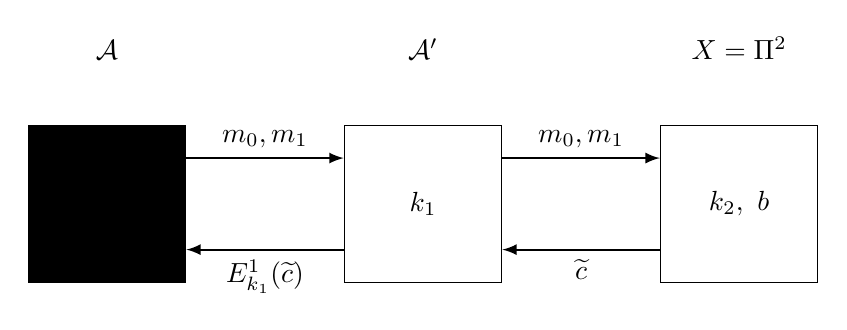
\begin{tikzpicture}[node distance=2cm,scale=1,box/.style={draw,shape=rectangle,minimum width=2cm,minimum height=2cm}]
   \node[box,fill=black    ] (A)    {                } ;
   \node[box,right=of A    ] (A')   { $k_1$          } ;
   \node[box,right=of A'   ] (Pi 2) { $k_2,~b$       } ;
   \node[above=2em of A    ]        { $\mathcal  { A } $        } ;
   \node[above=2em of A'   ]        { $\mathcal  { A } ^\prime$ } ;
   \node[above=2em of Pi 2 ]        { $X=\Pi^2$      } ;
   \draw[thick,>=latex,->] (A.30)     -- node[above] {$m_0,m_1$} (A'.150);
   \draw[thick,>=latex,->] (A'.30)    -- node[above] {$m_0,m_1$} (Pi 2.150);
   \draw[thick,>=latex,->] (Pi 2.210) -- node[below] {$\widetilde{c}$} (A'.-30);
   \draw[thick,>=latex,->] (A'.210)   -- node[below] {$E^1_{k_1}(\widetilde{c})$} (A.-30);
\end{tikzpicture}
\end{center}
\caption{Ablauf des hypothetischen Angriffs}
\label{fig:angriff}
\end{figure}

\end{document}
